\section{Overview}
Sentiment and emotion analysis are two closely related yet distinct fields within natural language processing (NLP) and computational linguistics, aiming to interpret human affective states from textual data. Sentiment analysis typically focuses on determining the polarity—whether an expressed opinion is positive, negative, or neutral. In contrast, emotion analysis captures more nuanced affective states that mirror human psychological experiences. A pivotal contribution to the study of emotions was provided by \citet{ekman1992there}, who identified six fundamental emotions—joy, anger, sadness, fear, surprise, and disgust—recognized across cultures. These basic emotions have laid the groundwork for much of the research in the area, serving as a universal framework for categorizing affective expressions in text.
\newline

This chapter offers an overview of existing studies on sentiment and emotion analysis, outlining methods that utilize textual, visual, and multimodal data. Section~\ref{sec:text_analysis} introduces text-based approaches, covering both classical machine learning and modern deep learning techniques. Section~\ref{sec:vision_analysis} turns to vision-based emotion analysis, focusing on methods for extracting affective cues from images.
Section~\ref{sec:multimodal_analysis} explores multimodal sentiment and emotion analysis, detailing fusion strategies that integrate textual and visual inputs.
Recognizing the challenges of large-scale annotation, Section~\ref{sec:weakly_supervised_back} discusses weakly supervised learning approaches relevant to both text and vision domains.
Finally, Section~\ref{sec:summary} summarizes key findings and highlights research gaps that shape the objectives of this thesis.


\section{Text-Based Sentiment and Emotion Analysis}
\label{sec:text_analysis}

Text-based sentiment and emotion analysis has been a cornerstone of NLP research for several decades, driven by applications such as customer feedback monitoring, social media analysis, and mental health assessment. Over time, methods in this field have evolved from simple, lexicon-driven approaches to sophisticated deep neural architectures capable of capturing subtle linguistic cues.

\subsection*{Lexicon-Based Methods}
Among the earliest techniques in sentiment and emotion analysis are lexicon-based methods, which rely on pre-compiled dictionaries where each word is assigned a sentiment polarity or emotion score. For instance, the word \textit{happy} might carry a positive sentiment score, while \textit{sad} might be scored as negative. An exemplar resource in this category is SentiWordNet \cite{baccianella-etal-2010-sentiwordnet}, an extension of the WordNet lexical database augmented with sentiment scores for synonym sets (synsets).
\newline

These methods are prized for their simplicity and interpretability, but they also have clear limitations. They often require additional linguistic preprocessing—handling negation (e.g., \textit{not happy}), intensifiers (e.g., \textit{very happy}), and modifiers (e.g., \textit{slightly happy})—to ensure accurate sentiment and emotion classification. Because they rely on static word scores, lexicon-based methods can struggle with context-dependent meaning, slang, or domain-specific jargon.

\subsection*{Classical Machine Learning Approaches}
As NLP advanced, researchers moved toward more data-driven approaches. Classical machine learning algorithms—such as Naïve Bayes, Support Vector Machines (SVMs), and Logistic Regression—became widely adopted for sentiment and emotion classification. These models are typically trained on labeled datasets in which each text snippet is annotated with a sentiment (positive, negative, neutral) or an emotion category.
\newline

Feature engineering plays a pivotal role in these methods, where textual features like word n-grams, part-of-speech (POS) tags, and syntactic or semantic cues are extracted to represent documents numerically. While these handcrafted features can be effective, the performance of classical algorithms often depends heavily on their quality. Moreover, these models lack a robust mechanism for automatically learning contextual representations, a key limitation that paved the way for neural network-based approaches.

\subsection*{Deep Learning and Neural Networks}
A paradigm shift occurred with the advent of deep learning, which moved away from manual feature design toward automatically learned representations of text. Early neural architectures for sentiment and emotion analysis leveraged Recurrent Neural Networks (RNNs) \cite{Mikolov:2010wx}. RNNs process sequential data by maintaining a hidden state that is updated at each time step, allowing the model to capture the influence of earlier words on later ones within a sentence.
\newline

However, vanishing and exploding gradients in standard RNNs prompted the development of more robust variants like Long Short-Term Memory (LSTM) \cite{10.1162/neco.1997.9.8.1735} and Gated Recurrent Units (GRUs) \cite{cho2014learningphraserepresentationsusing}. These architectures alleviate gradient-related issues, making them particularly well-suited for modelling long-range dependencies in text. Bidirectional RNNs \cite{1556215} further enhanced the capacity to integrate context by processing text in both forward and backward directions.

\subsection*{Convolutional Neural Networks (CNNs) for Text}
In parallel, researchers began adapting Convolutional Neural Networks (CNNs) originally developed for image processing to NLP tasks \cite{10.5555/2999134.2999257}. By applying one-dimensional convolutions over word embeddings, CNNs effectively capture local n-gram features within short windows of text. The most salient features are then combined via pooling layers for subsequent classification.
\newline

Despite strong performance on various benchmarks, CNNs are less effective at modeling long-range dependencies due to their local, filter-based architecture. As tasks increasingly demanded a more global understanding of context, attention-based mechanisms and transformer architectures began to dominate the field.

\subsection*{Attention Mechanisms and Transformers}
A major leap in sentiment and emotion analysis came with attention mechanisms \cite{Bahdanau2014NeuralMT}, which allow the model to focus selectively on the most pertinent words or phrases. By weighting different parts of the input according to their relevance, attention enhances both performance and interpretability, offering insights into why a certain sentiment or emotion is assigned.
\newline

Building on attention mechanisms, the Transformer architecture \cite{vaswani2023attentionneed} eliminated the need for recurrent processing, using instead a self-attention mechanism that captures contextual relationships across all positions in a sequence. Transformers yield contextualized embeddings that have proven invaluable for tasks like sentiment and emotion classification.

\subsection*{Pretrained Language Models and Fine-Tuning}
Modern NLP is increasingly shaped by pretrained language models such as BERT \cite{DBLP:journals/corr/abs-1810-04805} and GPT \cite{Radford2018ImprovingLU}, which learn general-purpose linguistic representations from massive corpora. These models can be fine-tuned for specific tasks, including sentiment and emotion analysis, often by adding a simple classification layer.
\newline

RoBERTa \cite{DBLP:journals/corr/abs-1907-11692} refines the BERT pretraining process by eliminating the next-sentence prediction objective, using dynamic masking, and training on longer sequences with larger batches and more data. As a result, RoBERTa routinely achieves state-of-the-art results across several NLP benchmarks.
\newline

Tailored toward social media data, BERTweet \cite{nguyen-etal-2020-bertweet} is the first large-scale pretrained language model specifically optimized for English Tweets. Built on the RoBERTa architecture, it outperforms strong baselines in downstream tasks like sentiment analysis, irony detection, and named-entity recognition of emerging entities, showcasing how domain-focused pretraining can significantly boost performance.
\newline

Additional variants such as DistilBERT \cite{sanh2020distilbertdistilledversionbert} and T5 \cite{raffel2023exploringlimitstransferlearning} further streamline and enhance transformer-based models by adjusting training objectives, data settings, or network sizes. Although these powerful models have substantially advanced text-based sentiment and emotion analysis, challenges remain, particularly in capturing domain-specific nuances and in effectively integrating multimodal inputs (e.g., combining text with images). Ongoing research thus explores domain adaptation, transfer learning, and multimodal analysis to push the boundaries of what text-based approaches can achieve.

\section{Vision-Based Sentiment and Emotion Analysis}
\label{sec:vision_analysis}

Historically, sentiment and emotion analysis has been dominated by text-based methods. However, vision-based approaches have gained prominence due to their ability to capture facial expressions, body language, and other visual cues that are difficult to infer from text alone. Such cues are especially critical in domains where textual data is sparse, ambiguous, or unavailable—for instance, in video surveillance or human-computer interaction—making vision-based sentiment analysis a powerful complementary method.
\newline

The potential impact of vision-based methods spans various fields. In healthcare, for example, analyzing visual data can help monitor patients’ emotional well-being and provide early interventions \cite{6940284}. Despite these advantages, vision-based sentiment analysis faces unique hurdles such as variations in lighting, pose, occlusion, and cultural differences in emotional expression \cite{10.1145/3240508.3240574}. These challenges have spurred ongoing research into more robust and context-sensitive techniques.

\subsection*{Traditional Feature Extraction}

Early work in vision-based sentiment analysis relied on handcrafted feature extraction to detect low-level visual patterns indicative of emotional states. Popular methods included the Scale-Invariant Feature Transform (SIFT) \cite{Lowe2004DistinctiveIF} and the Histogram of Oriented Gradients (HOG) \cite{1467360}, which identify edges, corners, and gradients. These features are subsequently fed into classical machine learning algorithms (e.g., SVMs or KNNs) to infer emotions.
\newline

While such approaches are computationally efficient and interpretable, their reliance on predefined descriptors limits their ability to capture high-level semantics and subtle emotional nuances \cite{6940284}. For example, distinguishing between a genuine smile and a forced one, or recognizing complex emotions like confusion, often lies beyond the capability of handcrafted features. As these limitations became more apparent, researchers began exploring data-driven techniques to automatically learn more expressive features.

\subsection*{Convolutional Neural Networks (CNNs)}

A significant leap forward occurred with the rise of Convolutional Neural Networks (CNNs) \cite{lecun_deep_2015}. Unlike handcrafted feature methods, CNNs learn hierarchical representations of visual data, extracting both low-level features (e.g., edges, textures) and high-level semantic information (e.g., facial expressions, emotional context). This shift drastically improved performance in emotion recognition and set a new standard in vision-based analysis.
\newline

The watershed moment for CNNs was the introduction of AlexNet in 2012 \cite{10.5555/2999134.2999257}, which showcased the effectiveness of deep convolutional layers in feature learning. Subsequent architectures—such as VGGNet \cite{simonyan2015deepconvolutionalnetworkslargescale}, Inception \cite{szegedy2015rethinkinginceptionarchitecturecomputer}, and ResNet \cite{he2015deepresiduallearningimage}—further refined deep learning techniques, tackling issues like the vanishing gradient problem and allowing for very deep network structures. These innovations led to state-of-the-art accuracy in identifying emotions from facial expressions and other visual cues.
\newline

One advantage of CNNs is the feasibility of transfer learning, where models pretrained on large-scale datasets like ImageNet \cite{5206848} are fine-tuned on specific tasks. This process can yield strong performance in sentiment analysis, even with relatively small labeled datasets \cite{yosinski2014transferablefeaturesdeepneural}. For instance, a CNN pretrained on ImageNet can be adapted to recognize facial expressions by retraining its final layers on a curated dataset of facial images.

\subsubsection*{Recent CNN-Based Advances}
Recent studies have adapted CNN-based architectures to capture more contextual or fine-grained emotional information. For example, \citet{limami_contextual_2024} address contextual emotion detection by proposing two deep learning models—a Deep Convolutional Neural Network (DCNN) and a VGG19-based model—that jointly leverage 26 discrete emotion categories and three continuous emotional dimensions (valence, arousal, dominance). This strategy integrates both body and contextual features, achieving a mean Average Precision (mAP) of up to 79.60\%. Their work underscores the importance of context in interpreting subtle emotional states.
\newline

Another novel approach is SmileyNet \cite{al-halah2020}, which exploits emoji-based embeddings to overcome the limited size of sentiment datasets. By gathering 4 million images from Twitter, annotated with emojis, the authors trained a deep network to predict these emojis, thereby creating sentiment-aligned embeddings. This embedding outperformed traditional object-based representations (e.g., ImageNet) in visual sentiment analysis and fine-grained emotion classification. Furthermore, hybrid architectures that combine Multi-Scale Dynamic 1D CNNs with Gated Transformers have been shown to be highly effective in EEG-based emotion recognition, demonstrating the value of fusing spatial-spectral features with global dependencies \cite{cheng_eeg-based_2024}.
\newline

Despite their success, CNNs also come with notable challenges. They can be computationally expensive to train, especially as depth increases (e.g., ResNet \cite{he2015deepresiduallearningimage}), and they sometimes struggle to capture long-range global relationships within an image. These limitations have paved the way for alternative architectures, particularly those built on transformers.

\subsection*{Vision Transformers (ViTs)}

The latest advancements in vision-based sentiment analysis have been driven by \textbf{Vision Transformers (ViTs)} \cite{dosovitskiy2021imageworth16x16words} and their variants, such as \textbf{Swin Transformers} \cite{liu2021swintransformerhierarchicalvision}. Unlike CNNs, which process images through convolutional filters, ViTs treat images as sequences of patches and apply self-attention mechanisms to capture global relationships within the visual data. This approach enables a more comprehensive understanding of complex emotional expressions, particularly in scenarios where subtle cues are critical.
\newline

ViTs were initially inspired by the success of transformers in natural language processing (NLP), where self-attention mechanisms have proven highly effective at modeling long-range dependencies in text \cite{vaswani2023attentionneed}. By adapting this architecture to visual data, ViTs can capture both local and global features, making them particularly well-suited for tasks like emotion recognition, where context and fine-grained details are important \cite{dosovitskiy2021imageworth16x16words}. For example, a ViT can analyze the relationship between different facial regions (e.g., eyes, mouth, and eyebrows) to infer emotions like surprise or disgust.
\newline

One of the most notable variants of ViTs is the Swin Transformer, which introduces a hierarchical feature extraction process. Swin Transformers divide an image into non-overlapping windows and apply self-attention within each window, reducing computational complexity while maintaining the ability to capture global relationships. This hybrid approach combines the strengths of ViTs and traditional CNNs, enabling state-of-the-art performance on various benchmarks. 
\newline

ViTs have also paved way for multi-modal approaches such as \textbf{CLIP (Contrastive Language-Image Pretraining)} \cite{radford2021learningtransferablevisualmodels} have shown remarkable potential in tasks that involve vision and language integration. This capability is particularly relevant for emotion recognition tasks that rely on both visual cues and associated text, such as social media posts containing images and captions.
\newline

The success of ViTs and their variants, along with multi-modal models like CLIP, has opened up new possibilities for vision-based sentiment analysis. These models are particularly effective at handling complex scenarios, such as group emotion recognition or the analysis of subtle micro-expressions \cite{liu2021swintransformerhierarchicalvision}. \citet{soni_vision_2024} apply a ViT-based model was applied to the FER-2013 dataset for emotion detection in human-computer interaction (HCI). The study emphasized meticulous preprocessing, data augmentation, and fine-tuning of the ViT model, achieving a testing accuracy of 70\%. However, they also come with challenges, including high computational costs and the need for large amounts of training data. Future research is likely to focus on improving the efficiency and scalability of these models, as well as exploring their application in real-world settings.


\section{Multimodal Sentiment and Emotion Analysis}
\label{sec:multimodal_analysis}

Multimodal sentiment/emotion analysis is a rapidly evolving field focused on understanding human emotions by integrating data from multiple modalities, such as text, audio, and visual inputs. Because human communication naturally spans these different modalities, relying on a single source of information often results in incomplete or inaccurate emotion recognition. As a result, multimodal approaches are increasingly critical for achieving more robust and comprehensive emotion analysis. 

\subsection{Multimodal Models}

A variety of multimodal models have been proposed to address the challenges of sentiment and emotion analysis. These approaches often combine textual and visual information to capture complementary cues that improve recognition accuracy. Below, we highlight four representative models that illustrate different strategies for integrating and aligning multimodal data.

\subsubsection{VisualBERT}
VisualBERT~\cite{li2019visualbertsimpleperformantbaseline} is a transformer-based architecture designed for vision-language tasks. It unifies visual and textual inputs within the same transformer encoder, leveraging BERT's bidirectional attention mechanism to process image regions and text tokens jointly. VisualBERT has shown strong performance in tasks such as visual question answering and image captioning. However, it relies on aligned image-text pairs during training, which constrains its flexibility in scenarios where perfectly paired multimodal data may be limited.

\subsubsection{MuAL: Multimodal Sentiment Analysis with Cross-Modal Attention and Difference Loss}
MuAL~\cite{deng_mual_2024} addresses the need for robust cross-modal representations specifically in sentiment analysis. By incorporating cross-modal attention and a difference loss to reduce the gap between image and text representations, MuAL outperforms traditional unimodal methods and demonstrates strong transfer-learning capabilities. Notably, it remains effective even when its pre-trained parameters are frozen, highlighting its potential for real-world applications where computational efficiency and generalization are crucial.

\subsubsection{MULSER: Multi-Level Semantic Reasoning Network}
While some multimodal approaches focus on broad sentiment categories (e.g., positive vs.\ negative), MULSER~\cite{9920172} targets fine-grained emotion classification, such as differentiating between ``happiness'' and ``love.'' The model employs graph attention networks to build multi-level graphs for images (object-level, global-level, and joint regional-global) and word-level graphs for text. A cross-modal attention fusion module then integrates the enriched visual and textual features. The resulting framework achieves state-of-the-art accuracy and F1 scores, underscoring the importance of sophisticated semantic reasoning and cross-modal interaction for nuanced emotion detection.

\subsubsection{CLIP}
CLIP (Contrastive Language–Image Pre-training) is a neural network model that aligns textual and visual modalities within a shared embedding space. This alignment enables various multimodal tasks without the need for task-specific labelled datasets. Departing from traditional supervised learning approaches that rely on domain-specific annotations, CLIP employs a zero-shot learning paradigm, allowing it to generalize across tasks by capturing the relationships between text and images without explicit fine-tuning \cite{radford2021learningtransferablevisualmodels}.
\newline

CLIP is trained using a contrastive learning objective that maximizes the cosine similarity for matched image-text pairs while minimizing it for mismatched pairs. By doing so, CLIP learns representations that effectively capture semantic relationships across modalities. This capability allows the model to perform tasks such as image classification by comparing embedded textual labels (e.g., “a photo of a dog”) with image embeddings in a shared latent space. Figure \ref{fig:sidebyside} illustrates the contrastive learning framework employed in CLIP.
\newline

\begin{figure}[h]
\centering
\begin{minipage}[b]{0.48\textwidth}
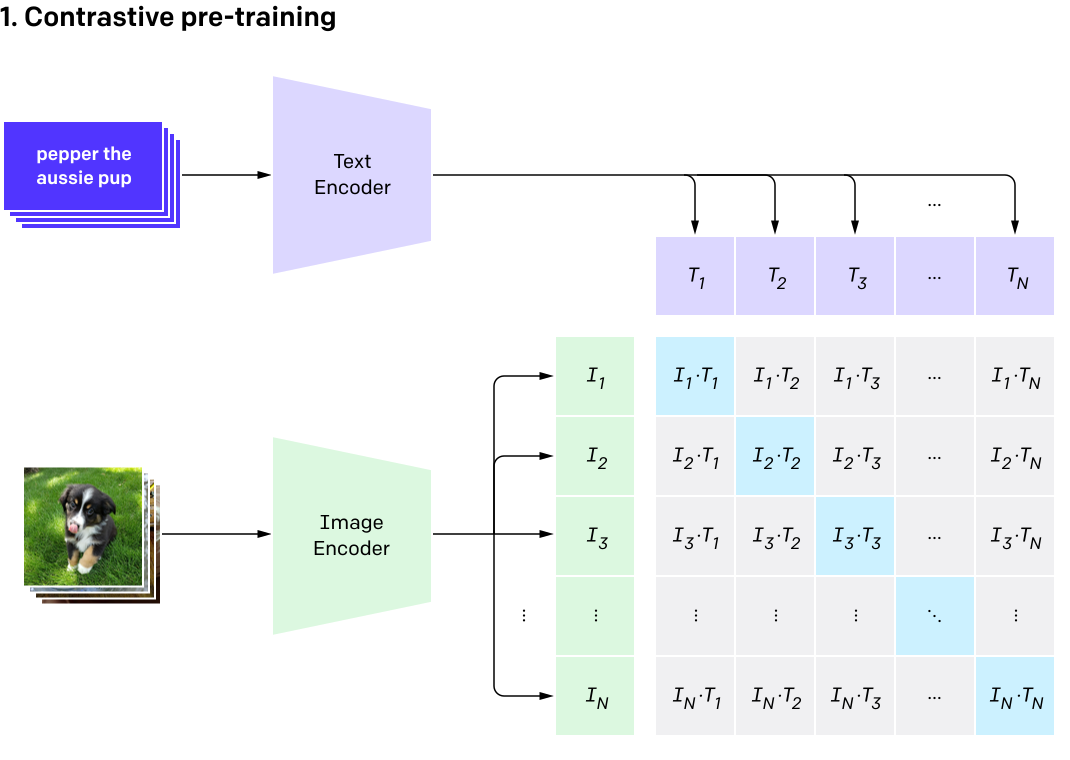
\includegraphics[width=\textwidth]{images/overview-a-clip.png}
\caption{Contrastive Pre-training}
\label{fig:contrastive_loss }
\end{minipage}
\hfill
\begin{minipage}[b]{0.45\textwidth}
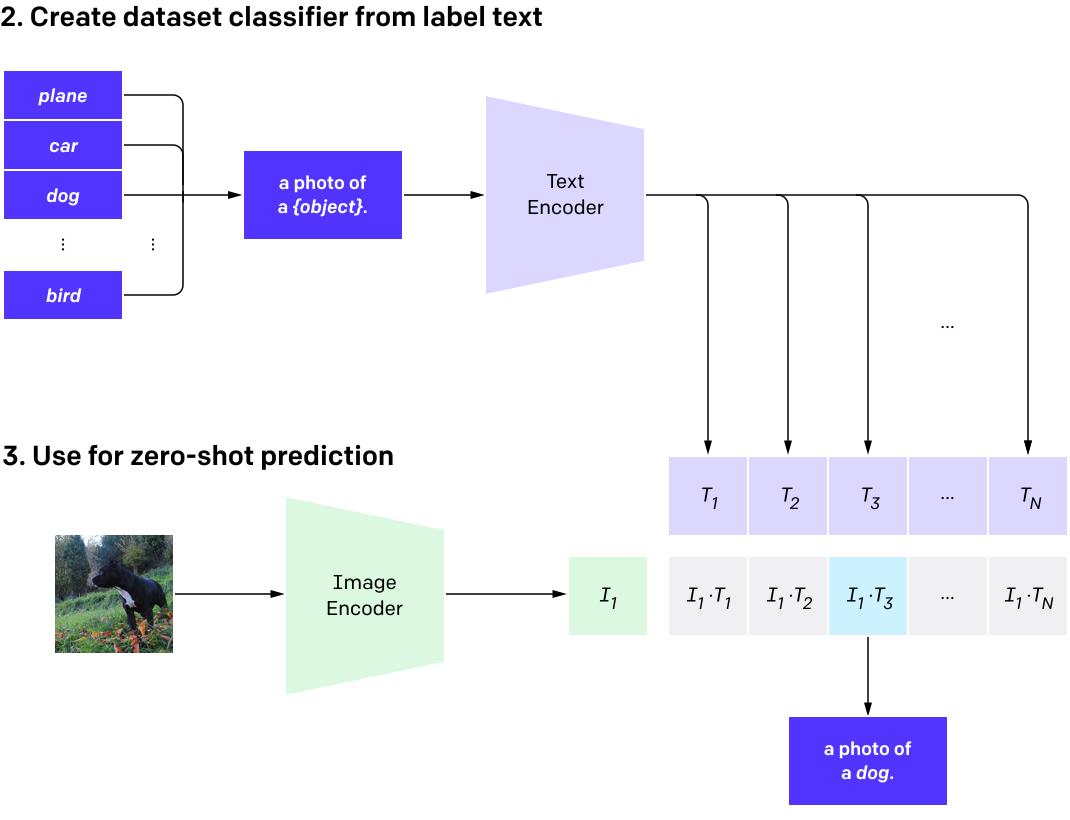
\includegraphics[width=\textwidth]{images/overview-b-clip.png}
\caption{Creation of dataset classifier and final prediction}
\label{fig:clip_zero }
\end{minipage}
\caption{Approach to training CLIP and Inference \cite{radford2021learningtransferablevisualmodels}}
\label{fig:sidebyside}
\end{figure}

CLIP was trained on approximately 400 million image-text pairs collected from the internet, leveraging the natural co-occurrence of images and their descriptions instead of manual annotations. This large and diverse dataset allows the model to learn broad visual-textual relationships, making it applicable to a variety of tasks. CLIP’s architecture consists of two main components: an image encoder (commonly a Vision Transformer \cite{dosovitskiy2021imageworth16x16words}) and a text encoder (based on transformer architectures like GPT or BERT \cite{Radford2018ImprovingLU, DBLP:journals/corr/abs-1810-04805}). Both encoders produce high-dimensional embeddings that are projected into a shared latent space, where contrastive learning aligns matched image-text pairs and separates mismatched ones.
\newline

To further improve generalization, CLIP leverages data augmentation techniques—such as resizing, cropping, and color adjustments—and large batch sizes that provide a diverse set of negative examples during contrastive learning. One of CLIP’s most significant strengths is its zero-shot learning paradigm, which allows the model to interpret natural language as a “programming interface.” In this setup, text prompts are embedded into the shared latent space and compared to image embeddings. Tasks like image classification, object detection, and text-based image retrieval can thus be performed without any task-specific fine-tuning (Figure \ref{fig:clip_zero }).
\newline

CLIP’s foundational principles have informed other multimodal models, such as LXMERT \cite{tan2019lxmertlearningcrossmodalityencoder}, which employs cross-attention mechanisms for visual question answering and image captioning. These advances extend CLIP’s core ideas to a variety of multimodal applications, including affective computing and social media analysis.
\newline

Through these examples, we see how multimodal models vary in their approaches to data alignment, representation learning, and zero-shot inference. However, each faces common challenges in effectively combining heterogeneous sources of information. In the next section, we review broader fusion strategies that address these challenges more generally.

\subsection{Fusion Strategies}

In addition to designing specialized architectures, researchers have explored general strategies for effectively integrating multiple data streams. This topic has garnered increasing attention due to the growing availability of diverse data sources, including text, images, audio, and video. Two key surveys offer comprehensive overviews of multimodal alignment and fusion techniques:

\begin{itemize}
    \item \textbf{Pawlowski et al.\ (2023):} In ``Effective Techniques for Multimodal Data Fusion: A Comparative Analysis'' \cite{pawlowski_effective_2023}, the authors systematically evaluate the performance of different fusion paradigms, ranging from early to late fusion, and highlight the trade-offs in computational cost and representational power.
    \item \textbf{Li et al.\ (2024):} In ``Multimodal Alignment and Fusion: A Survey'' \cite{li_multimodal_2024}, the authors discuss alignment mechanisms, such as cross-attention and co-attention, as well as the role of contrastive objectives in bridging modalities. The survey also addresses practical considerations like data imbalance and missing modalities.
\end{itemize}

These analyses underline the importance of aligning representations from each modality before fusing them, as well as the potential benefits of modular architectures that can be tailored to domain-specific needs. By leveraging strategies drawn from these studies, researchers can build models that not only detect broad sentiments but also distinguish subtle emotional nuances from noisy, unstructured real-world data.


\subsubsection{Fusion Techniques and Their Applications}
Researchers have proposed various techniques to integrate data from multiple modalities effectively. In particular, two influential studies by Pawlowski et al.\ and Li \& Tang provide comprehensive analyses of fusion strategies, each emphasizing different facets of multimodal data integration.

\paragraph{Pawlowski et al. (2023).}
focus on three primary fusion techniques—\textbf{late fusion}, \textbf{early fusion}, and \textbf{sketch representation}—and evaluate their effectiveness in classification tasks. Their findings highlight the dominance of \textbf{late fusion} in scenarios where one modality is dominant or when unimodal models already perform well. For instance, in the Amazon Reviews dataset, late fusion achieved the highest accuracy (0.969) by combining textual and visual modalities at the decision level, making it robust against modality-specific noise.
\newline

In contrast, \textbf{early fusion} integrates modalities by concatenating their embeddings at the input level, which can be advantageous when modalities are highly interdependent. However, Pawlowski et al.\ observe that early fusion often underperforms compared to late fusion. This pattern is notably evident in the MovieLens datasets, where the merged embeddings sometimes lead to information loss or redundancy, especially if one modality is less informative.
\newline

The \textbf{sketch representation} technique, which maps each modality into a lower-dimensional common space via hash functions, offers a memory-efficient alternative. While it underperforms on classification accuracy relative to the other methods, its scalability makes it attractive for large-scale systems (e.g., recommendation engines). Pawlowski et al.\ underscore the importance of selecting a fusion approach that aligns with task requirements, modality impact, and memory constraints.

\paragraph{Li \& Tang (2024).}
Building on these ideas, Li \& Tang propose a broader taxonomy by categorizing fusion strategies into \textbf{encoder-decoder fusion}, \textbf{kernel-based fusion}, \textbf{graphical fusion}, and \textbf{attention-based fusion}. Each method aims to exploit inter-modal relationships to improve performance on tasks that combine text, images, audio, and other data sources.
\newline

\textbf{Encoder-Decoder Fusion.} In this approach, each modality is first processed by a separate encoder to produce latent representations, which are then merged by a decoder. This strategy is particularly suited for tasks like image captioning and video summarization, where the goal is to generate coherent outputs (e.g., natural language descriptions) from multiple input types \cite{8269806}.
\newline

\textbf{Attention-Based Fusion.} Attention mechanisms have gained widespread popularity due to their ability to selectively weight the importance of features across modalities. Li \& Tang highlight the effectiveness of models like ALBEF (Align Before Fuse) and BLIP (Bootstrapped Language-Image Pretraining) \cite{li2021alignfusevisionlanguage, li2022blipbootstrappinglanguageimagepretraining}, which first align modalities before fusing them in a joint latent space. These techniques are especially valuable in social media analytics and emotion recognition, where subtle interactions among text, images, and audio can significantly influence the outcome \cite{poria_review_2017}.

\subsubsection{Alignment Challenges and Conclusion}
Despite these advancements, aligning heterogeneous data sources remains a critical challenge. Li \& Tang distinguish between \textbf{explicit alignment} methods (e.g., Dynamic Time Warping, Canonical Correlation Analysis) and \textbf{implicit alignment} approaches (e.g., attention mechanisms, GANs, and VAEs). Explicit methods are especially useful for tasks requiring precise temporal or spatial synchronization (e.g., video-audio alignment), whereas implicit methods learn a shared latent space that can adapt to incomplete or noisy inputs.
\newline

Both Pawlowski et al.\ and Li \& Tang underscore the need for robust, scalable frameworks to handle the growing volume and complexity of multimodal datasets. Challenges such as modal feature misalignment, varying data quality, and high computational costs persist. Furthermore, the limited contribution of certain modalities (as observed with visual data in the MovieLens case) highlights the importance of selecting the most informative data sources. Future research will benefit from standardized benchmarks, akin to GLUE in NLP, and the continued development of adaptive methods—such as attention-based and graphical fusion techniques—to effectively integrate diverse data modalities at scale.



\section{Weakly Supervised Learning}
\label{sec:weakly_supervised_back}
Weakly supervised learning (WSL) has emerged as a critical area of research in machine learning, addressing scenarios where labelled data is scarce, noisy, or incomplete. This section reviews recent advancements in WSL, focusing on its applications in both computer vision and natural language processing (NLP). The discussion is organized into two main subsections: \emph{Weakly Supervised Learning in Text} and \emph{Weakly Supervised Learning in Vision}, followed by a critical analysis of the limitations and future directions of WSL.

\subsection{Weakly Supervised Learning in Text}

Weakly supervised learning has also been extensively applied to NLP tasks, particularly in scenarios where annotated data is scarce or expensive to obtain. Recent work has focused on generating supervision signals from weak sources, such as language models or heuristic rules.
\newline

\citet{song_learning_2022} in the paper \emph{Learning from Noisy Labels with Deep Neural Networks: A Survey}, provide a comprehensive review of techniques for training deep neural networks (DNNs) in the presence of noisy labels. The main techniques discussed in the paper are categorized into five groups:

\subsubsection*{1. Robust Architecture}
\begin{itemize}
    \item \textbf{Noise Adaptation Layer:} Adds a layer to model the noise transition matrix, which helps in learning the label transition behavior. This approach aims to mimic the label transition process by estimating the probability of label corruption.
    \item \textbf{Dedicated Architecture:} Designs specialized architectures to handle more complex noise types, such as instance-dependent noise. These architectures often involve multiple networks or human-assisted constraints to improve robustness.
\end{itemize}

\subsubsection*{2. Robust Regularization}
\begin{itemize}
    \item \textbf{Explicit Regularization:} Modifies the expected training loss to prevent overfitting. Techniques in this category often involve bilevel optimization, pre-training, or gradient clipping to control overfitting to noisy labels.
    \item \textbf{Implicit Regularization:} Introduces stochasticity to improve generalization. Methods like adversarial training, label smoothing, and mixup are used to encourage the model to learn more robust representations.
\end{itemize}

\subsubsection*{3. Robust Loss Function}
\begin{itemize}
    \item \textbf{Noise-Tolerant Loss Functions:} Modifies loss functions to be robust to label noise. These loss functions are designed to minimize the impact of noisy labels by ensuring that the loss remains stable even when labels are corrupted. Examples include mean absolute error (MAE) variants, generalized cross-entropy, and symmetric cross-entropy.
\end{itemize}

\subsubsection*{4. Loss Adjustment}
\label{subsubsec:loss_adjust}
\begin{itemize}
    \item \textbf{Loss Correction:} Adjusts the loss based on the estimated noise transition matrix. This involves correcting the loss values during forward or backward propagation to account for label noise.
    \item \textbf{Loss Reweighting:} Assigns different weights to examples based on their likelihood of being correctly labelled. This approach reduces the influence of potentially noisy examples during training.
    \item \textbf{Label Refurbishment:} Refurbishes noisy labels by combining them with model predictions. This technique dynamically updates the labels during training to reduce the impact of incorrect annotations.
    \item \textbf{Meta Learning:} Automates the process of loss adjustment using meta-learning techniques. These methods learn to reweight examples or adjust labels based on a small clean validation set.
\end{itemize}

\subsubsection*{5. Sample Selection}
\begin{itemize}
    \item \textbf{Multi-network Learning:} Uses multiple networks to identify clean examples. By leveraging disagreements between networks or using a mentor-student approach, these methods filter out noisy examples.
    \item \textbf{Multi-round Learning:} Iteratively refines the set of clean examples over multiple training rounds. This approach gradually improves the quality of the selected examples by repeatedly training and filtering.
    \item \textbf{Hybrid Approach:} Combines sample selection with other techniques like semi-supervised learning. These methods treat selected examples as clean labelled data and the remaining examples as unlabelled, applying semi-supervised learning to improve robustness.
\end{itemize}

\subsubsection*{Additional Topics}
\begin{itemize}
    \item \textbf{Noise Rate Estimation:} Techniques for estimating the noise rate, including using the noise transition matrix, Gaussian Mixture Model (GMM), and cross-validation.
    \item \textbf{Experimental Design:} Discussion of publicly available datasets and evaluation metrics used to validate robust training methods.
    \item \textbf{Future Research Directions:} Identifies areas for future research, such as instance-dependent label noise, multi-label data with label noise, class imbalance data with label noise, robust and fair training, connection with input perturbation, and efficient learning pipelines.
\end{itemize}

The paper provides a detailed comparison of these methods based on six properties: flexibility, no pre-training, full exploration, no supervision, heavy noise, and complex noise. It also discusses the challenges and future directions in the field of learning from noisy labels.
\newline

\citet{chen_multiple_2022} propose a framework called \emph{Multiple Weak Supervision (MWS)} for short text classification, addressing challenges such as insufficient labelled data, data sparsity, and imbalanced classification. MWS leverages multiple weak supervision sources, including keyword matching, regular expressions, and distant supervision clustering, to automatically label unlabelled data. The framework generates probabilistic labels through a conditional independent model, which helps mitigate class imbalance. Evaluated on public, synthetic, and real-world datasets, MWS demonstrates significant improvements in recall and F1-scores without compromising precision. This work highlights the potential of combining multiple weak supervision sources to address the challenges of short text classification.
\newline

\citet{zeng_weakly_2022} introduce a novel approach for weakly supervised text classification that leverages a masked language model (MLM) to generate supervision signals. By appending the sentence ``This article is talking about [MASK]'' to documents, the MLM's predictions for the [MASK] token are used as weak supervision signals. These generated words are then used to train a latent variable model called \emph{WDDC (Word Distribution and Document Classifier)}, which learns a word distribution over predefined categories and a document classifier without requiring annotated data. Evaluated on datasets like AGNews, 20Newsgroups, and UCINews, the method outperforms existing weakly supervised baselines by 2\%, 4\%, and 3\%, respectively. This work demonstrates the potential of using MLMs to generate supervision signals for text classification tasks in low-resource settings.
\newline

\citet{gera_zero-shot_2022} in the paper \emph{"Zero-Shot Text Classification with Self-Training"} address the challenge of improving zero-shot text classification performance using self-training. Zero-Shot classification, where models classify text without task-specific labelled data, often underperforms compared to supervised models. The authors propose a self-training approach that fine-tunes zero-shot classifiers on their most confident predictions, leveraging only class names and an unlabelled dataset.
\newline

\subsubsection*{Key Contributions and Findings}

\begin{itemize}
    \item \textbf{Self-Training for Zero-Shot Models:} The authors adapt self-training, traditionally used in semi-supervised learning, to improve general-purpose zero-shot models. This involves generating pseudo-labels from the model's confident predictions and iteratively fine-tuning the model.
    
    \item \textbf{Entailment-Based Classification:} The study focuses on Natural Language Inference (NLI)-based models, which map text classification tasks to textual entailment problems. The authors hypothesize that self-training helps these models better understand class name interactions and the specific entailment sub-types relevant to the target task.
    
    \item \textbf{Experimental Setup:} The method is evaluated on eight diverse text classification datasets. The authors use three off-the-shelf NLI models (RoBERTa, DeBERTa, and BART) and demonstrate significant performance improvements across all datasets after self-training.
    
    \item \textbf{Token Masking:} To enhance the informativeness of pseudo-labelled examples, the authors introduce a token masking heuristic that masks tokens most similar to the class name, forcing the model to rely on other contextual cues.
    
    \item \textbf{Cross-Task Effects:} The study explores the impact of self-training on one task for performance on another. Results show that self-training on related tasks (e.g., within the same domain) can be beneficial, while unrelated tasks (e.g., sentiment vs. emotion classification) may degrade performance.
    
    \item \textbf{Practical Implications:} The approach requires only a modest amount of unlabelled data (up to 10K examples) and does not need domain expertise, making it accessible for practitioners.
\end{itemize}


The paper concludes that self-training is a valuable tool for adapting general-purpose zero-shot models to specific tasks, offering significant performance gains with minimal effort. This work opens avenues for further research into combining self-training with other zero-shot learning paradigms and exploring its applicability to different types of NLP tasks.


\subsection{Weakly Supervised Learning in Vision}

Weakly supervised learning has been widely adopted in computer vision tasks, particularly in scenarios where obtaining large-scale, high-quality labelled datasets is prohibitively expensive. Several approaches have been proposed to leverage noisy or incomplete labels effectively.
\newline

\citet{hu_weakly_2019} propose a novel framework for weakly supervised image classification in the presence of noisy labels. Their method, which consists of a clean net and a residual net, leverages both clean and noisy labelled data to improve classification performance. The clean net learns a mapping from the feature space to the clean label space, while the residual net models the residual mapping between clean and noisy labels, acting as a regularization term to prevent overfitting. Evaluated on multi-label (OpenImage \cite{openimages}, MS COCO \cite{lin2015microsoftcococommonobjects}) and single-label (Clothing1M \cite{7298885}) datasets, the approach demonstrates significant improvements in mean average precision (mAP) and top-1 accuracy. This work highlights the importance of effectively utilizing noisy data in weakly supervised learning and provides a robust framework for handling label noise in practical applications.
\newline

\citet{mahajan_exploring_2018} explore the limits of weakly supervised pretraining by leveraging billions of Instagram images labelled with hashtags. Their study shows that models pretrained on such large-scale, weakly supervised datasets outperform those pretrained on traditional datasets like ImageNet in transfer learning tasks, including image classification and object detection. Key findings include the robustness of models to label noise, the importance of aligning source and target label spaces, and the potential of ``hashtag engineering'' to improve transfer learning results. This work underscores the value of leveraging naturally annotated, large-scale datasets for pretraining deep learning models.
\newline

\citet{xie_self-training_2020} introduce \emph{Noisy Student Training}, a semi-supervised learning method that enhances model performance by leveraging unlabelled data. The approach involves training a teacher model on labelled data, generating pseudo-labels for unlabelled data, and then training a larger or equal-sized student model on both labelled and pseudo-labelled data while injecting noise (e.g., dropout, stochastic depth, and data augmentation). This method achieves state-of-the-art results on ImageNet \cite{5206848}, with an 88.4\% top-1 accuracy, and demonstrates significant improvements in robustness on challenging datasets like ImageNet-A \cite{hendrycks2021naturaladversarialexamples}, ImageNet-C, and ImageNet-P \cite{hendrycks2019benchmarkingneuralnetworkrobustness}. The study highlights the effectiveness of combining weakly supervised learning with semi-supervised techniques to improve both accuracy and robustness.


\subsection*{Limitations}

Despite its promise, weakly supervised learning (WSL) has notable limitations. \citet{zhu_weaker_2023} critically assess the effectiveness of WSL approaches, arguing that their benefits are often overestimated. Their experiments on eight NLP datasets reveal that fine-tuning models on even minimal clean validation data (e.g., five samples per class) often outperforms sophisticated WSL methods. Moreover, WSL fails to improve over weak labels without clean validation samples, and its advantages diminish when clean data is used for training instead of validation. 


\section{Summary}
\label{sec:summary}
This chapter reviewed existing work on sentiment and emotion analysis, emphasizing text-based, vision-based, and multimodal approaches. Text-based methods primarily rely on transformer-based architectures such as BERT and GPT, which have demonstrated state-of-the-art performance in sentiment and emotion classification tasks. Vision-based approaches leverage convolutional neural networks (CNNs) and vision transformers to extract emotion-relevant features from images, often using facial expressions or scene context.
\newline

Multimodal sentiment and emotion analysis integrates textual and visual data, improving predictive performance by capturing complementary cues from both modalities. Fusion strategies, such as early, late, and hybrid fusion, play a crucial role in effectively combining different modalities. Despite these advancements, one of the major challenges remains the scarcity of labelled data, which limits the generalization of supervised models. To address this, weakly supervised learning techniques have been explored, particularly in text and vision domains, leveraging noisy or incomplete labels to train models effectively.
\newline

The literature highlights the strengths and limitations of various approaches, underscoring the need for improved multimodal models and better weakly supervised learning strategies. These insights inform the research direction of this thesis, which aims to enhance emotion analysis through advanced multimodal techniques and more effective label-learning methods.
